\documentclass{article}
\usepackage[utf8]{inputenc}
\usepackage{graphicx}
\usepackage{xurl}
\graphicspath{{./images/}}

\title{Assessing the accessibility components in the Moodle platform architecture to propose improvements based on WCAG guidelines.}
\author{Amanda Bermudez, Gerardo Salas Montoya}
\date{\today}



\begin{document}

\maketitle

\section{Objective}
The main objective of this study is to evaluate the accessibility components of the Moodle e-learning platform and provide improvement recommendations based on the application of WCAG guidelines (version 2.2).

\section{Specific Objectives}
\begin{enumerate}
    \item Analyze the current accessibility components of the Moodle platform at Universidad Cenfotec. This analysis aims to obtain an initial diagnosis of the situation by reviewing industry best practices.
    \item Compare the principles and accessibility criteria established in WCAG 2.2 to determine their relevance and effectiveness for improving Moodle's accessibility.
    \item Develop recommendations based on the conducted research to address the most critical accessibility issues of Moodle at Universidad Cenfotec.
\end{enumerate}

\section{Introduction}
Following the pandemic, we have experienced significant changes in various aspects of our lives, such as access to information, social interaction, educational methods, and work environments. Virtualization has become a reality in nearly all fields, presenting a considerable challenge for the general population and especially for individuals with disabilities in the educational sector.

In numerous institutions, educational platforms have undergone a notable transition: from being a sparingly used resource to becoming the primary channel of interaction between students and educators. However, due to the sudden context of this digitalization, many institutions were not fully prepared and were forced to implement accelerated changes. Unfortunately, these changes do not always meet basic accessibility standards, which may exclude certain groups of people with disabilities.

Depending on the ease of accessing information on the main webpage, users typically decide whether to continue navigating those websites or not (Acosta-Vargas, Luján-Mora, \& Salvador-Ullauri, 2016). In the case of institutional platforms, users do not have the freedom to decide whether to continue navigating as it becomes essentially obligatory since it becomes an indispensable tool for their educational process.

According to OMS, one in every six people has some form of disability, totaling approximately 1.3 billion people worldwide (World Health Organization, 2023). In Costa Rica, according to the National Disability Survey (ENADIS), in 2018, there were over 670,000 individuals over 18 years old with some form of disability (National Institute of Statistics and Census of Costa Rica [INEC] and National Council for Persons with Disabilities [CONAPDIS], 2018, p.60). In this context, this survey is the first of its kind and aims to measure the prevalence of disability for the formulation, monitoring, and evaluation of public policies, which is a clear example that although we have taken the first steps on this important path, we still have a long way to go to ensure that all people, regardless of their abilities, can fully access the services and resources available in our society.

In 2019, Directive (051-MTSS-MICITT) includes compliance with the accessibility criteria established by the Web Content Accessibility Guidelines (WCAG) in its version 2.1 for the Costa Rican public sector at the first level, with the exception of the Legislative and Judicial Powers. It excludes some public institutions and provides a grace period of 3 years (Costa Rican Executive Branch, 2019).

Despite regulatory efforts, through an evaluation conducted by the Ministry of Science, Innovation, Technology, and Telecommunications of 388 websites of evaluated institutions, it was evidenced that "86.60\% do not comply with the minimum accessibility standards to achieve basic accessibility (A) rating" (quoted in PROSIC, 2022, p.42).

Notably, private institutions currently have no obligation to adhere to the WCAG guidelines within their websites. In the context of education, this lack of obligation poses a significant challenge. Therefore, this project aims to consolidate a proposal for improving the institutional webpage of Universidad Cenfotec.

\section{Research Questions.}
This section lists the main research questions that we set out to answer.
\begin{itemize}
    \item Is the Moodle platform of University Cenfotec meeting the principles of accessibility outlined in WCAG 2.2?
    \item How can we improve the web accessibility of Universidad Cenfotec's Moodle by incorporating the main needs identified by the WCAG 2.2 guidelines to promote greater inclusion in the web ecosystem of Universidad Cenfotec?
\end{itemize}

\section{Background}
Many authors consider LMSs and their accessibility from different points of view. When the accessibility in context of e-learning is considered, many authors highlighted that there is a need to define criteria for instructors, authors of the contents and e-learning specialist that create and run activities on the web (Bocevska et al,2018).

Given that this research is conducted within the legal context of Costa Rica, we will adopt the definition of accessibility provided in Directive 051-MTSS-MICITT (Costa Rican Executive Branch, 2019). This directive defines accessibility as "the measures adopted by public and private institutions to ensure that persons with disabilities have access, on equal terms with others, to the physical environment, transportation, information and communications, including information and communication technologies and systems, and to other services and facilities open to the public or for public use. These measures also include the identification and removal of such barriers."

\section{Related Work}
The following research has been conducted focusing on web accessibility within the context of e-learning software architecture

In 2018, Schiavone published an article titled "An analysis through experiences in scientific literature and a case study," where the focus is on analyzing the accessibility of the Moodle online learning platform, reviewing previous studies and evaluating the accessibility of specific Moodle installations (Schiavone, A., 2018).

Acosta and Luján-Mora in 2016 conducted a comparative study of three Learning Management Systems (LMS), Moodle, Sakai, and the system called ABC, developed in Ecuador to evaluate the levels of accessibility according to users' needs. They analyzed and compared the selected LMSs based on accessibility criteria, considering functional tasks on a scale with 6 levels of accessibility that can be used for decision-making and LMS selection from the perspective of teachers and students (Lujan, et al., 2016).

Boceveska, Savoska, Risvestki, and Blazeska in 2018 published the research "Analysis of Accessibility of the e-Learning Platforms According to the WCAG 2.0 Standard Compliance," which aims to analyze the accessibility of the latest public versions of several Learning Management Systems (LMS), such as Moodle, Eliademy, Docebo, Sakai, and ATutor, for people with disabilities. The analysis will evaluate compliance with different levels of criteria established in the Web Content Accessibility Guidelines (WCAG).

The web accessibility project of the University of Costa Rica focuses on the application of international web accessibility standards, specifically on the WCAG 2.1 standard. Throughout the document, there is a reference to the importance of complying with these standards to ensure that websites are accessible to all users, including people with disabilities (Da Silva Bermúdez, K., García Sibaja, J., Martínez de Lemos, F. J., Matarrita Brenes, P., Ureña Benavides, K., \& Vargas Varela, J.).

We also find the publication "AccGuideLiner: Towards a Modelling Approach of Web Accessibility Requirements following WCAG 2.2," which describes a detailed model for describing accessibility requirements by integrating expert knowledge and domain knowledge to simplify its implementation in tools. The document is aimed at web developers, designers, accessibility engineers, and researchers who wish to understand the guidelines and accessible requirements from the technical perspective to the code phase.

The main source of information is the guidelines established by WCAG 2.2 developed by the World Wide Web Consortium (W3C), which set technical standards and guidelines for creating more accessible web content for a wide range of users, including those with disabilities. These guidelines address key aspects such as perception, operability, and understanding of web content, ensuring it is accessible for both assistive technologies and users without disabilities.

\section{IBM equal accessibility checker}
To collect the WCAG 2.2 ratings on the analyzed pages, we used the "IBM Equal Accessibility Checker 7.3," which is an open-source tool (https://github.com/IBMa/equal-access) and available for free. It integrates into the browser's development tools and provides a comprehensive analysis environment through the auditor's or developer's browser, allowing for automatic accessibility evaluation of the visited page.This study is conducted using Google Chrome, and therefore, the tool is obtained through the official Google Chrome extension store.

We will use version 7.3, which includes six new success criteria from the Web Content Accessibility Guidelines (WCAG) 2.2 Level A and AA, as well as criteria that were already included in previous versions.

The rule set applied in this tool is grouped as follows:

\begin{itemize}
    \item Non-text content
    \item Keyboard content
    \item Language Parsing
\end{itemize}

The technique used for analysis relies on the tool's functionality, which checks various aspects of web accessibility in accordance with WCAG 2.2 guidelines, as mentioned earlier. It scans the pages to be analyzed, pinpointing potential accessibility issues and offering insights into elements that don't meet specified standards, such as exporting results in Excel format, among other functionalities.

Key features to note include:

\begin{itemize}
    \item Automatic scanning: The tool automatically analyzes the webpage, identifying areas of concern regarding accessibility.
    \item Comprehensive reports: Following the analysis, we thoroughly examine the detailed reports provided by the tool to draw conclusions and formulate recommendations aimed at improving accessibility.
\end{itemize}

The URL that will be covered in the scope of the investigation are in the taxonomy of the page in image

\begin{figure}[h]
    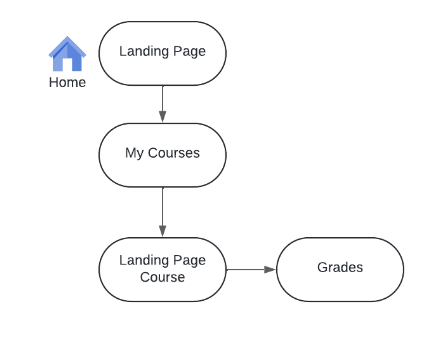
\includegraphics[width=0.9\textwidth]{images/figure1.png}
    \caption{Moodle page taxonomy}
    \label{fig:figure1}
\end{figure}

\section{Analysis and Results}
The W3 Consortium provides a publicly available quick reference for objectively rating the integration of accessibility into a platform. The WCAG 2.2 guidelines have a list of categories that can be rated on three levels: A, AA, and AAA. The lowest category, A, indicates poor accessibility, while the AA category signifies meeting all criteria of the A rating plus additional criteria. The highest category, AAA, implies that the previous levels are met.

We have established tree levels to categorize the issue founded in the analysis.


\section{Conclusions}
Here are the conclusions about the .....

\section*{Bibliography/References}

\begin{itemize}
    \item Instituto Nacional de Estadísticas y Censos de Costa Rica, y Consejo Nacional de Personas con Discapacidad. (2018). \textit{Encuesta Nacional sobre Discapacidad 2018}. Instituto Nacional de Estadísticas y Censos (INEC). Retrieved from \url{https://admin.inec.cr/sites/default/files/media/reenadis2018_2.pdf}
    \item Organización Mundial de la Salud. (2023, 7 de marzo). \textit{Discapacidad}. WHO. Recuperado el 18 de marzo, 2024, de \url{https://www.who.int/es/news-room/factsheets/detail/disability-and-health}
    \item Bocevska, A., Savoska, S., Ristevski, B., \& Blazheska-Tabakovska, N. (2018). \textit{Analysis of accessibility of the e-learning platforms according to the WCAG 2.0 standard compliance}.
    \item Da Silva Bermúdez, K., García Sibaja, J., Martínez de Lemos, F. J., Matarrita Brenes, P., Ureña Benavides, K., \& Vargas Varela, J. Volviendo accesible la accesibilidad web: creación de un modelo de aplicación de accesibilidad web que propicie el uso de los estándares internacionales de la WCAG en usuarios especializados del área de diseño y desarrollo de sitios web en Costa Rica.
    \item Schiavone, A. G. (2018). Is Moodle accessible? An analysis through experiences in scientific literature and a case study. In Proceedings of (Vol. 1).
    \item S-COM: Davinsson Nunjar Flores. (n.d.-b). Sistema Costarricense de Información Jurídica. S-COM. \url{https://www.pgrweb.go.cr/scij/Busqueda/Normativa/Normas/nrm_texto_completo.aspx?param1=NRTC&nValor1=1&nValor2=89061&nValor3=116705&strTipM=T}
    \item Ara, J., \& Sik-Lanyi, C. (2023, May). AccGuideLiner: Towards a Modelling Approach of Web Accessibility Requirements following WCAG 2.2. In 2023 IEEE International Conference on Smart Information Systems and Technologies (SIST) (pp. 10-15). IEEE.
    \item Acosta-Vargas, P., Luján-Mora, S., \& Salvador-Ullauri, L. (2016). Evaluación de la accesibilidad de las páginas web de las universidades ecuatorianas.
    \item Eggert, E., \& Abou-Sahra, S. (2023, November 12). How to meet WCAG. \url{https://www.w3.org/WAI/WCAG22/quickref/?versions=2.1}.
    \item University of California. (n.d.). Electronic accessibility. UCOP. \url{https://www.ucop.edu/electronic-accessibility/standards-and-best-practices/levels-of-conformance-a-aa-aaa.html#:~:text=WCAG%202.0%20guidelines%20are%20categorized,%2C%20and%20AAA%20(highest)}.
    \item \url{https://www.kerwa.ucr.ac.cr:8443/bitstream/handle/10669/89666/VOLVIENDO%20ACCESIBLE%20LA%20ACCESIBILIDAD%20WEB%20CREACI%c3%93N%20DE%20UN%20MODELO%20DE%20APLICACI%c3%93N%20DE%20ACCESIBILIDAD%20WEB%20QUE%20PROPICIE%20EL%20USO%20DE%20LOS%20EST%c3%81NDARES%20INTERNACIONALES%20DE%20LA%20WCAG%20EN%20USUARIOS%20ESPECIALIZADOS%20DEL%20%c3%81REA%20DE%20DISE%c3%91O%20Y%20DESARROLL.pdf?sequence=4&isAllowed=y}.
    \item Tania Acosta, Sergio Luján-Mora, Comparison from The Levels Of Accessibility on LMS Platforms that Supports the Online Learning System, 8th International Conference on Education and New Learning Technologies, pp. 2704-2711, Barcelona, Spain, 2016, doi: 10.21125/edulearn.2016.1579, \url{https://library.iated.org/view/ACOSTA2016COM}.
\end{itemize}


\end{document}

